\documentclass[UTF8,zihao=-4]{ctexart}
\usepackage[a4paper,margin=2.1cm]{geometry}
\usepackage{array}
\usepackage{longtable}
\usepackage{hyperref}
\usepackage{verbatim}
\usepackage{graphicx}
\usepackage{tikz}
\usetikzlibrary{arrows.meta,positioning,fit,calc,shapes.geometric}
\hypersetup{hidelinks}
\setlength{\parindent}{0pt}
\setlength{\parskip}{0.55em}
\renewcommand{\arraystretch}{1.22}
\setlength{\tabcolsep}{3pt}
\emergencystretch=4em
\sloppy
\title{02 需求工程复习讲义}
\author{}
\date{}
\begin{document}
\maketitle
\tableofcontents
\newpage


整理范围：

\begin{itemize}
\item \texttt{PPT/02-01-需求工程基础.pdf}
\item \texttt{PPT/02-02-AI辅助需求获取.pdf}
\item \texttt{PPT/02-03-用例建模与用户故事.pdf}
\item \texttt{PPT/02-04-需求分析与AI辅助建模.pdf}
\item \texttt{PPT/02-05-需求文档化验证与冲突检测.pdf}
\end{itemize}

交叉参考：

\begin{itemize}
\item \texttt{Exam/2012.pdf}：销售用例分析类图。
\item \texttt{Exam/2013A.pdf}：ATM 业务需求、用户需求、系统级需求、功能需求与非功能需求。
\item \texttt{Exam/2013B.pdf}：ATM 用例图和系统顺序图。
\item \texttt{Exam/2014.pdf}：图书馆系统用例建模、用例顺序图到分析类图。
\item \texttt{Exam/2016.pdf}：支付宝支付用例图、概念类图。
\item \texttt{Exam/2020.pdf}：采购补货用例、需求分类、概念类图。
\item \texttt{Exam/2022.pdf}：校园卡自助系统用例、充值需求、概念类图。
\item \texttt{Exam/2025.pdf}：判断需求级别和需求类型、从用户级需求到系统级需求。
\item \texttt{Review/summary-重点.pdf}、\texttt{Review/Final\_Reference.pdf}：需求分类、用例粒度、概念类图、顺序图、状态图、SRS。
\end{itemize}

说明：

\begin{itemize}
\item 本部分是考试综合题最多的部分之一。答题重点不是画图好看，而是概念、关系、边界、粒度和可验证性正确。
\item AI 相关内容按“生成初稿 + 人工审查”的工程流程理解，不把 AI 输出直接当作需求结论。
\end{itemize}

\section{二、5 个课件的主线}

{
\footnotesize
\begin{longtable}{|>{\raggedright\arraybackslash}p{0.30\textwidth}|>{\raggedright\arraybackslash}p{0.30\textwidth}|>{\raggedright\arraybackslash}p{0.30\textwidth}|}
\hline
\textbf{课件} & \textbf{主线} & \textbf{必会关键词} \\
\hline
\endfirsthead
\hline
\textbf{课件} & \textbf{主线} & \textbf{必会关键词} \\
\hline
\endhead
\texttt{02-01} 需求工程基础 & 需求层次、需求类型、问题域 & 业务需求、用户需求、系统级需求、功能需求、非功能需求 \\
\hline
\texttt{02-02} AI 辅助需求获取 & AI 如何辅助访谈、整理和检查需求 & Prompt、利益相关者、隐含约束、人工审查 \\
\hline
\texttt{02-03} 用例建模与用户故事 & 从用户目标到用例图和用例描述 & Actor、Use Case、include、extend、前置条件、后置条件 \\
\hline
\texttt{02-04} 需求分析与 AI 辅助建模 & 从需求文本到分析模型 & 概念类图、顺序图、状态图、OCL \\
\hline
\texttt{02-05} 需求文档化验证与冲突检测 & SRS、追踪、验证与冲突处理 & SRS、可验证性、追踪矩阵、歧义、冲突、Spec \\
\hline
\end{longtable}
}


\bigskip\hrule\bigskip

\section{2. 需求工程}

\section{2.1 需求工程的含义}

需求工程覆盖所有围绕需求展开的活动。

核心活动：

\begin{itemize}
\item 需求获取
\item 需求分析
\item 需求规格说明
\item 需求验证
\item 需求管理
\end{itemize}

需求工程不是简单“问用户要功能”。它需要理解问题域、利益相关者、业务流程、约束条件、数据规则和外部系统。

\section{2.2 问题域}

问题域包含：

\begin{itemize}
\item 业务目标
\item 业务流程
\item 领域术语
\item 组织规则
\item 相关人员
\item 现有系统
\item 数据对象
\item 外部约束
\end{itemize}

需求工程的关键是先理解问题域，再定义系统边界和解决方案。

\section{2.3 需求层次}

\subsection{业务需求}

回答“为什么建设系统”。

关注：

\begin{itemize}
\item 战略目标
\item 业务价值
\item 愿景
\item 范围
\end{itemize}

示例：

\begin{quote}
建设校园卡自助系统，提高充值、挂失、查询等业务的自助化比例，降低人工窗口压力。
\end{quote}

\subsection{用户需求}

回答“用户想用系统完成什么任务”。

特点：

\begin{itemize}
\item 面向用户任务
\item 语言不够精确
\item 常混合功能、界面和约束
\end{itemize}

示例：

\begin{quote}
学生希望在网页或移动端自助完成校园卡充值，并查看充值记录。
\end{quote}

\subsection{系统级需求}

回答“系统必须提供什么能力和约束”。

特点：

\begin{itemize}
\item 精确
\item 可验证
\item 可追踪
\item 面向系统交互和响应
\end{itemize}

示例：

\begin{quote}
系统接收充值请求后，应校验校园卡状态和支付结果；支付成功后创建充值记录并更新账户余额。
\end{quote}

\section{2.4 需求类型}

Review 中常用两级分类：

{
\footnotesize
\begin{longtable}{|>{\raggedright\arraybackslash}p{0.30\textwidth}|>{\raggedright\arraybackslash}p{0.30\textwidth}|>{\raggedright\arraybackslash}p{0.30\textwidth}|}
\hline
\textbf{分类层次} & \textbf{类型} & \textbf{说明} \\
\hline
\endfirsthead
\hline
\textbf{分类层次} & \textbf{类型} & \textbf{说明} \\
\hline
\endhead
总体需求 & 项目需求 & 人员、成本、时间、交付物、计划约束。 \\
\hline
总体需求 & 过程需求 & 开发方法、协作方式、文档提交、持续集成、评审要求。 \\
\hline
总体需求 & 系统需求 & 软件、硬件和外部系统共同承担的系统能力。 \\
\hline
总体需求 & 其他需求 & 培训、人力、硬件采购、部署环境等配套要求。 \\
\hline
软件需求 & 功能、性能、质量属性、对外接口、约束、数据需求 & 直接描述软件产品要做什么、做到什么质量、遵守什么限制。 \\
\hline
\end{longtable}
}


\subsection{功能需求}

说明系统做什么。

示例：

\begin{itemize}
\item 查询校园卡余额。
\item 提交充值订单。
\item 查询充值记录。
\item 挂失校园卡。
\end{itemize}

说明：登录和权限校验通常服务于安全性质量属性，不作为普通业务用例；认证系统本身作为考试题目时，登录才作为该系统的核心功能。

\subsection{非功能需求}

说明系统达到什么质量或约束。

常见维度：

\begin{itemize}
\item 性能
\item 安全
\item 可用性
\item 可靠性
\item 可维护性
\item 可移植性
\item 易用性
\end{itemize}

性能维度：

\begin{itemize}
\item 速度
\item 容量
\item 吞吐量
\item 负载
\item 时效性或实时性
\end{itemize}

\subsection{外部接口需求}

说明系统与外部系统、硬件、用户界面之间的交互约束。

示例：

\begin{itemize}
\item 与支付平台通过 HTTPS 通信。
\item 与校园卡中心系统同步余额。
\item 前端通过 REST API 调用后端服务。
\end{itemize}

\subsection{约束}

说明系统建设必须遵守的限制。

示例：

\begin{itemize}
\item 使用学校统一身份认证。
\item 数据库存储在校内数据中心。
\item 后端采用 Java Spring Boot。
\end{itemize}

\subsection{数据需求}

说明系统需要管理的数据对象、数据字段、完整性规则和保留策略。

示例：

\begin{itemize}
\item 充值记录包含记录编号、校园卡号、金额、支付渠道、支付状态、创建时间。
\item 充值金额必须大于 0。
\end{itemize}

\section{2.5 AI 辅助需求获取}

AI 适合：

\begin{itemize}
\item 从访谈记录中提取功能点。
\item 整理用户故事。
\item 生成需求文档初稿。
\item 把自然语言改写成结构化条目。
\item 检查编号、格式和冲突线索。
\end{itemize}

AI 的薄弱点：

\begin{itemize}
\item 容易遗漏隐含业务规则。
\item 容易忽略系统边界。
\item 容易生成不符合真实组织流程的功能。
\item 对领域例外、权限规则、历史系统接口理解不足。
\end{itemize}

推荐流程：

\begin{enumerate}
\item Prompt：给出背景、角色、范围、输出格式。
\item Generate：生成需求条目或模型草图。
\item Review：人工核对业务规则、边界、异常和术语。
\item Refine：补充约束、优先级、验收标准和追踪关系。
\end{enumerate}

\bigskip\hrule\bigskip

\section{2.6 用例建模}

用例描述系统与外部对象之间的一组交互行为。它从用户目标出发，描述系统如何向参与者提供有价值的服务。

Cockburn 的区分：

\begin{itemize}
\item 用例：包含一个用户目标下的所有场景。
\item 场景：用例中的一条具体路径。
\end{itemize}

\subsection{基本元素}

\begin{itemize}
\item 参与者 Actor：系统外部与系统交互的角色。
\item 用例 Use Case：系统提供的服务。
\item 系统边界：区分系统内部和外部。
\item 关系：关联、包含、扩展、泛化。
\end{itemize}

参与者可以是人、外部系统、硬件设备或定时器。参与者位于系统边界外，用例位于系统边界内。

\subsection{include 与 extend}

include：

\begin{itemize}
\item 基本用例每次执行时都要执行被包含用例。
\item 方向：基本用例指向被包含用例。
\item 用于抽取多个用例共享的公共行为。
\end{itemize}

extend：

\begin{itemize}
\item 扩展用例在特定条件下插入基本用例。
\item 方向：扩展用例指向基本用例。
\item 用于异常、可选、附加行为。
\end{itemize}

示例：

\begin{itemize}
\item “充值” include “身份验证”：每次充值都要验证用户身份。
\item “充值失败处理” extend “充值”：只有支付失败或写入余额失败时触发。
\end{itemize}

\subsection{用例粒度}

合格用例通常满足：

\begin{itemize}
\item 对应一个业务事件。
\item 由参与者发起。
\item 在连续时间内完成。
\item 对参与者有业务价值。
\end{itemize}

常见错误：

\begin{itemize}
\item 把增删改查拆成太细的技术操作。
\item 把同一业务目标拆散。
\item 把登录、数据校验、数据库连接当作独立业务用例。
\item 在用例图里写实现细节。
\end{itemize}

\subsection{Cockburn 层次}

\begin{itemize}
\item 概要层：范围太大，适合说明系统目标。
\item 用户目标层：最适合作为主用例。
\item 子功能层：粒度较小，常用于 include 或内部步骤。
\end{itemize}

\section{2.7 用例描述模板}

十项模板：

\begin{enumerate}
\item 用例编号
\item 用例名称
\item 参与者
\item 触发条件
\item 前置条件
\item 后置条件
\item 基本流程
\item 扩展流程
\item 特殊需求
\item 备注
\end{enumerate}

前置条件是用例开始前已经成立的系统状态，不是“用户输入账号密码”这类步骤。

示例：充值用例简表

{
\footnotesize
\begin{longtable}{|>{\raggedright\arraybackslash}p{0.45\textwidth}|>{\raggedright\arraybackslash}p{0.45\textwidth}|}
\hline
\textbf{项目} & \textbf{内容} \\
\hline
\endfirsthead
\hline
\textbf{项目} & \textbf{内容} \\
\hline
\endhead
用例编号 & UC-Recharge \\
\hline
用例名称 & 校园卡充值 \\
\hline
参与者 & 持卡人 \\
\hline
触发条件 & 持卡人选择充值功能 \\
\hline
前置条件 & 持卡人已通过身份认证，校园卡状态正常 \\
\hline
后置条件 & 充值成功时账户余额增加，并生成充值记录 \\
\hline
基本流程 & 选择充值金额；系统创建充值订单；调用支付接口；支付成功后更新余额；显示结果 \\
\hline
扩展流程 & 支付失败时记录失败原因并提示用户；校园卡状态异常时拒绝充值 \\
\hline
特殊需求 & 充值结果写入和记录生成保持一致 \\
\hline
\end{longtable}
}


\section{2.8 用户故事与 BDD}

用户故事常用格式：

\begin{quote}
作为 \texttt{<角色>}，我想要 \texttt{<能力>}，以便 \texttt{<业务价值>}。
\end{quote}

示例：

\begin{quote}
作为持卡人，我想要在线充值校园卡，以便在食堂和门禁场景继续使用校园卡。
\end{quote}

BDD 使用 Given-When-Then：

\begin{quote}
\footnotesize
\begin{verbatim}
Given 持卡人已登录且校园卡状态正常
When 持卡人提交 100 元充值并完成支付
Then 系统增加校园卡余额并生成一条成功充值记录
\end{verbatim}
\end{quote}

ATDD 强调先定义验收测试，再驱动设计和实现。

\bigskip\hrule\bigskip

\section{2.9 需求分析模型}

常用模型：

\begin{itemize}
\item 用例图
\item 概念类图
\item 顺序图
\item 状态图
\item ER 图
\item OCL 约束
\end{itemize}

面向对象需求分析输出：

\begin{itemize}
\item 用例图和用例描述
\item 概念类图或领域模型
\item 顺序图
\item 状态图
\item OCL 约束
\end{itemize}

\section{2.10 概念类图}

概念类图描述问题域中的概念及其关系，属于分析模型。

它与设计类图的区别：

{
\footnotesize
\begin{longtable}{|>{\raggedright\arraybackslash}p{0.30\textwidth}|>{\raggedright\arraybackslash}p{0.30\textwidth}|>{\raggedright\arraybackslash}p{0.30\textwidth}|}
\hline
\textbf{项目} & \textbf{概念类图} & \textbf{设计类图} \\
\hline
\endfirsthead
\hline
\textbf{项目} & \textbf{概念类图} & \textbf{设计类图} \\
\hline
\endhead
阶段 & 需求分析 & 详细设计 \\
\hline
关注 & 领域概念 & 软件类、接口、方法 \\
\hline
内容 & 类名、属性、关联、多重性 & 属性、方法、可见性、接口、继承、依赖 \\
\hline
来源 & 用例、业务文本、领域知识 & 架构、设计原则、实现技术 \\
\hline
\end{longtable}
}


\subsection{从文本提取概念类}

步骤：

\begin{enumerate}
\item 收集用例描述、访谈记录和业务规则。
\item 标记名词和名词短语。
\item 合并同义词。
\item 删除纯属性、实现概念、外部系统、重复词和临时消息。
\item 与业务人员确认剩余概念。
\item 为概念添加属性、关联和多重性。
\end{enumerate}

判断一个词能否成为概念类：

\begin{itemize}
\item 系统需要长期记录它。
\item 它拥有多个属性。
\item 它参与业务规则。
\item 它与其他概念存在稳定关系。
\end{itemize}

示例：

\begin{itemize}
\item “充值记录”是概念类，因为系统要保存记录编号、金额、支付状态、时间等属性。
\item “金额”通常是属性，不是概念类。
\item “支付平台”是外部系统，在系统边界外。
\end{itemize}

\subsection{关联与多重性}

动词短语常提示关联：

\begin{itemize}
\item 用户拥有校园卡。
\item 校园卡产生充值记录。
\item 充值记录对应支付订单。
\end{itemize}

数量词提示多重性：

\begin{itemize}
\item 一个用户可以拥有多张校园卡。
\item 一张校园卡可以有多条充值记录。
\item 一条充值记录对应一个支付订单。
\end{itemize}

\section{2.11 顺序图}

顺序图描述对象之间按时间顺序发生的消息交互。

画法要点：

\begin{itemize}
\item 先选一个用例。
\item 从基本流程开始。
\item 每个交互步骤对应消息。
\item 使用 \texttt{alt} 表示分支，使用 \texttt{opt} 表示可选步骤。
\item 消息顺序必须与业务流程一致。
\end{itemize}

充值用例的典型对象：

\begin{itemize}
\item 持卡人
\item 充值界面
\item 充值控制器
\item 充值服务
\item 校园卡仓储
\item 充值记录仓储
\item 支付网关
\end{itemize}

典型流程：

\begin{enumerate}
\item 持卡人提交充值请求。
\item 控制器调用充值服务。
\item 服务查询校园卡状态。
\item 服务创建充值记录或充值订单。
\item 服务调用支付网关确认支付结果。
\item 服务更新余额。
\item 服务保存充值记录。
\item 控制器返回充值结果。
\end{enumerate}

\section{2.12 状态图}

状态图描述一个对象在生命周期内的状态变化。

适合建模：

\begin{itemize}
\item 订单
\item 校园卡
\item 支付记录
\item 设备
\item 会话
\end{itemize}

充值记录状态示例：

\begin{itemize}
\item Created
\item Paying
\item Success
\item Failed
\item Cancelled
\end{itemize}

状态图可以直接指导测试：

\begin{itemize}
\item 每条合法迁移对应一个测试。
\item 每条非法迁移对应一个异常测试。
\end{itemize}

\section{2.13 OCL}

OCL 是附着在 UML 模型上的声明式约束语言。

特点：

\begin{itemize}
\item 无副作用。
\item 说明不变式、前置条件和后置条件。
\item 可表达集合约束。
\end{itemize}

常见元素：

\begin{itemize}
\item \texttt{inv}：不变式。
\item \texttt{pre}：前置条件。
\item \texttt{post}：后置条件。
\item \texttt{@pre}：操作执行前的值。
\item \texttt{forAll}、\texttt{exists}、\texttt{select}、\texttt{collect}：集合操作。
\end{itemize}

示例：

\begin{quote}
\footnotesize
\begin{verbatim}
context Recharge
inv PositiveAmount:
  self.amount > 0
\end{verbatim}
\end{quote}

\begin{quote}
\footnotesize
\begin{verbatim}
context CampusCard::recharge(amount)
pre ValidAmount:
  amount > 0
post BalanceIncreased:
  self.balance = self.balance@pre + amount
\end{verbatim}
\end{quote}

\bigskip\hrule\bigskip

\section{2.14 SRS 与需求验证}

SRS 是系统级需求规格说明，从产品和系统视角列出需求。

用例文档和 SRS 的区别：

{
\footnotesize
\begin{longtable}{|>{\raggedright\arraybackslash}p{0.30\textwidth}|>{\raggedright\arraybackslash}p{0.30\textwidth}|>{\raggedright\arraybackslash}p{0.30\textwidth}|}
\hline
\textbf{项目} & \textbf{用例文档} & \textbf{SRS} \\
\hline
\endfirsthead
\hline
\textbf{项目} & \textbf{用例文档} & \textbf{SRS} \\
\hline
\endhead
视角 & 用户交互 & 系统能力 \\
\hline
组织方式 & 按用户目标 & 按功能、接口、数据、质量属性 \\
\hline
重点 & 场景和流程 & 可验证、可追踪的需求条目 \\
\hline
\end{longtable}
}


SRS 条目要使用刺激-响应结构：

\begin{quote}
当 \texttt{<刺激>} 发生时，系统应 \texttt{<响应>}。
\end{quote}

示例：

\begin{quote}
当持卡人完成支付且支付平台返回成功结果时，系统应更新校园卡余额并生成成功充值记录。
\end{quote}

\section{2.15 好需求的标准}

常见标准：

\begin{itemize}
\item 正确性
\item 完整性
\item 一致性
\item 可读性
\item 可修改性
\item 可验证性
\item 可追踪性
\end{itemize}

验证方法：

\begin{itemize}
\item 同行评审
\item 原型验证
\item 仿真
\item 测试用例推导
\item 追踪矩阵检查
\end{itemize}

\section{2.16 需求追踪}

前向追踪：

\begin{quote}
需求 → 设计 → 代码 → 测试
\end{quote}

后向追踪：

\begin{quote}
代码或设计 → 需求来源
\end{quote}

追踪矩阵常见列：

\begin{itemize}
\item 需求编号
\item 需求来源
\item 设计模块
\item 代码模块
\item 测试用例
\item 状态
\end{itemize}

需求属性：

\begin{itemize}
\item 编号
\item 描述
\item 理由
\item 来源
\item 优先级
\item 稳定性
\item 状态
\item 负责人
\item 版本
\item 变更历史
\end{itemize}

\section{2.17 歧义与冲突}

歧义类型：

\begin{itemize}
\item 词法歧义：同一词有多种含义。
\item 句法歧义：句子结构导致多种解释。
\item 语用歧义：上下文或业务背景不足导致理解不一致。
\end{itemize}

冲突类型：

\begin{itemize}
\item 直接矛盾：两个需求对同一条件给出相反响应。
\item 资源冲突：时间、预算、算力、设备或人员无法同时满足。
\item 优先级冲突：不同利益相关者对需求重要性排序不同。
\end{itemize}

处理流程：

\begin{enumerate}
\item 标记冲突需求编号。
\item 说明冲突类型。
\item 找到对应利益相关者。
\item 召开评审。
\item 记录决策和理由。
\item 更新 SRS、追踪矩阵和变更历史。
\end{enumerate}

\section{2.18 Spec 驱动开发}

SDD 链路：

\begin{quote}
Spec → Design → Tasks → Code
\end{quote}

好的 Spec 包含：

\begin{itemize}
\item 问题背景
\item 用户故事
\item 功能范围
\item 验收标准
\item 非功能约束
\item 不在范围内的内容
\item 待确认问题
\end{itemize}

在 AI 协作中，Spec 是人与 AI 之间的工程协议。Spec 越清晰，AI 输出越容易被审查、测试和接入项目。

\bigskip\hrule\bigskip

\section{对应考试模板}

\section{7.4 需求题答题模板}

\subsection{写业务需求}

\begin{quote}
\footnotesize
\begin{verbatim}
BR-01 建设校园卡自助系统，提高校园卡充值、查询、挂失等业务的
自助办理比例，减少人工窗口处理压力。
\end{verbatim}
\end{quote}

\subsection{写用户需求}

\begin{quote}
\footnotesize
\begin{verbatim}
UR-01 作为持卡人，我想在线充值校园卡，以便在余额不足时继续使用校园卡。
\end{verbatim}
\end{quote}

\subsection{写系统级功能需求}

\begin{quote}
\footnotesize
\begin{verbatim}
FR-01 当持卡人提交充值请求时，系统应校验持卡人身份、校园卡状态和充值金额。
FR-02 当支付平台返回支付成功结果时，系统应更新校园卡余额并生成成功充值记录。
FR-03 当持卡人查询充值记录时，系统应返回该校园卡的充值记录列表。
\end{verbatim}
\end{quote}

\subsection{写非功能需求}

\begin{quote}
\footnotesize
\begin{verbatim}
NFR-01 系统应通过 HTTPS 提供充值接口。
NFR-02 充值成功响应时间应不超过 3 秒，不包含第三方支付平台处理时间。
NFR-03 系统应记录每次充值请求、支付结果和余额更新结果。
\end{verbatim}
\end{quote}

\section{7.5 概念类图题模板}

校园卡系统概念类：

\begin{itemize}
\item User
\item CampusCard
\item RechargeRecord
\item PaymentOrder
\item LossReport
\item Transaction
\end{itemize}

主要关系：

\begin{itemize}
\item 一个 \texttt{User} 拥有零张或多张 \texttt{CampusCard}。
\item 一张 \texttt{CampusCard} 对应零条或多条 \texttt{RechargeRecord}。
\item 一条 \texttt{RechargeRecord} 对应一个 \texttt{PaymentOrder}。
\item 一张 \texttt{CampusCard} 对应零条或多条 \texttt{LossReport}。
\item 一张 \texttt{CampusCard} 对应零条或多条 \texttt{Transaction}。
\end{itemize}

概念类示例：

\begin{quote}
\footnotesize
\begin{verbatim}
User
  userId
  name
  studentNo

CampusCard
  cardNo
  balance
  status

RechargeRecord
  recordId
  amount
  status
  createdAt

PaymentOrder
  orderId
  channel
  status
  paidAt
\end{verbatim}
\end{quote}

\section{7.6 顺序图题模板}

充值基本流程：

\begin{quote}
\footnotesize
\begin{verbatim}
Actor -> RechargePage: 输入金额并提交
RechargePage -> RechargeController: POST 
/api/recharges
RechargeController -> RechargeService: 
recharge(command)
RechargeService -> CampusCardRepository: 
findByCardNo(cardNo)
CampusCardRepository --> RechargeService: 
CampusCard
RechargeService -> PaymentGateway: 
pay(order)
PaymentGateway --> RechargeService: 
PaymentResult
RechargeService -> CampusCard: 
recharge(amount)
RechargeService -> CampusCardRepository: 
save(card)
RechargeService -> RechargeRecordRepository:
 save(record)
RechargeService --> RechargeController: 
RechargeResult
RechargeController --> RechargePage: JSON 
result
\end{verbatim}
\end{quote}

异常分支：

\begin{itemize}
\item 校园卡不存在：抛出 \texttt{CardNotFoundException}。
\item 校园卡已挂失：返回充值拒绝。
\item 支付失败：保存失败记录并返回失败原因。
\item 保存余额失败：执行事务回滚并记录错误。
\end{itemize}

\section{7.7 状态图题模板}

校园卡状态：

\begin{quote}
\footnotesize
\begin{verbatim}
Normal -> Lost: reportLost
Lost -> Normal: cancelLossReport
Normal -> Frozen: freeze
Frozen -> Normal: unfreeze
Normal -> Cancelled: cancel
Lost -> Cancelled: cancel
Frozen -> Cancelled: cancel
\end{verbatim}
\end{quote}

充值记录状态：

\begin{quote}
\footnotesize
\begin{verbatim}
Created -> Paying: startPayment
Paying -> Success: paymentSucceeded
Paying -> Failed: paymentFailed
Created -> Cancelled: cancel
Failed -> Created: retry
\end{verbatim}
\end{quote}

测试点：

\begin{itemize}
\item 正常迁移要测。
\item 非法迁移要测。
\item 每个状态的允许操作要测。
\end{itemize}

\bigskip\hrule\bigskip

\section{高频考点展开}

\section{需求级别判断}

判断需求级别时，先看它回答的问题：

\begin{itemize}
\item 业务需求回答“为什么建系统”，对应组织目标和业务价值。
\item 用户需求回答“用户要完成什么任务”，对应用户目标和业务流程。
\item 系统级需求回答“系统接收什么输入、做什么处理、给出什么输出”，对应可实现、可测试、可追踪的系统行为。
\end{itemize}

示例：

\begin{quote}
\footnotesize
\begin{verbatim}
业务需求：提高校园卡充值和查询业务的自助办理比例。
用户需求：持卡人要在线完成校园卡充值并查看结果。
系统级需求：当支付平台返回支付成功结果时，系统应更新校园卡余额并生成充值记录。
\end{verbatim}
\end{quote}

\section{需求类型判断}

{
\footnotesize
\begin{longtable}{|>{\raggedright\arraybackslash}p{0.30\textwidth}|>{\raggedright\arraybackslash}p{0.30\textwidth}|>{\raggedright\arraybackslash}p{0.30\textwidth}|}
\hline
\textbf{需求表述} & \textbf{类型} & \textbf{判断依据} \\
\hline
\endfirsthead
\hline
\textbf{需求表述} & \textbf{类型} & \textbf{判断依据} \\
\hline
\endhead
系统应支持用户查询余额 & 功能需求 & 说明系统做什么 \\
\hline
充值结果应在 3 秒内返回 & 性能需求 & 说明响应时间 \\
\hline
系统通过 HTTPS 提供接口 & 对外接口需求或约束 & 说明外部通信方式 \\
\hline
金额字段只能包含数字且大于 0 & 数据需求 & 说明数据格式和取值范围 \\
\hline
系统应记录充值操作日志 & 功能需求，也服务于可审计性 & 说明系统行为 \\
\hline
\end{longtable}
}


需求表述要避免“很快”“方便”“尽量”等不可验证词。改写时使用具体条件、阈值、输入和输出。

\section{用例粒度判断}

合格用例的判断标准：

\begin{enumerate}
\item 由外部参与者触发。
\item 对参与者产生业务价值。
\item 在连续时间内完成。
\item 对应一个用户目标或业务事件。
\end{enumerate}

不适合作为业务用例的内容：

\begin{itemize}
\item 登录：通常是前置条件或 include，除非题目专门考认证系统。
\item 数据校验：属于步骤或规则。
\item 连接数据库：属于实现细节。
\item 点击按钮：属于界面动作，不是完整用户目标。
\end{itemize}

\section{概念类图答题步骤}

\begin{enumerate}
\item 从用例文本中提取名词和名词短语。
\item 删除属性词、动作词、界面词、临时消息和外部系统。
\item 保留系统需要长期记录并参与业务规则的概念。
\item 给每个概念补关键属性。
\item 根据动词短语补关联。
\item 根据数量词补多重性。
\end{enumerate}

示例：

\begin{quote}
\footnotesize
\begin{verbatim}
“一张校园卡可以有多条充值记录”：
CampusCard 1 ---- 0..* RechargeRecord
\end{verbatim}
\end{quote}

\section{顺序图答题步骤}

顺序图从一个用例的基本流程开始：

\begin{enumerate}
\item 左侧放参与者。
\item 按层次放界面、控制器、服务、仓储、外部接口。
\item 每个用例步骤转成一条消息。
\item 查询用返回虚线表示。
\item 异常流程用 \texttt{alt} 描述。
\end{enumerate}

评分点是消息顺序和职责边界，不是图形装饰。

\section{校园卡图形题示例}

用例图：


\begin{center}
\resizebox{0.9\textwidth}{!}{%
\begin{tikzpicture}[>=Stealth, actor/.style={draw, align=center, fill=gray!10}, usecase/.style={draw, ellipse, align=center, minimum width=30mm, minimum height=9mm, fill=blue!5}, node distance=10mm and 18mm]
\node[actor] (student) {持卡人};
\node[usecase, right=of student] (balance) {查询余额};
\node[usecase, below=of balance] (recharge) {校园卡充值};
\node[usecase, below=of recharge] (records) {查询充值记录};
\node[usecase, below=of records] (loss) {挂失校园卡};
\node[usecase, below=of loss] (detail) {查询消费明细};
\node[actor, right=36mm of recharge] (bank) {支付平台};
\node[actor, right=36mm of records] (center) {校园卡中心};
\foreach \u in {balance,recharge,records,loss,detail}{\draw[-] (student) -- (\u);}
\draw[-] (bank) -- (recharge);
\draw[-] (center) -- (balance);
\draw[-] (center) -- (recharge);
\end{tikzpicture}}
\end{center}



概念类图：


\begin{center}
\resizebox{0.92\textwidth}{!}{%
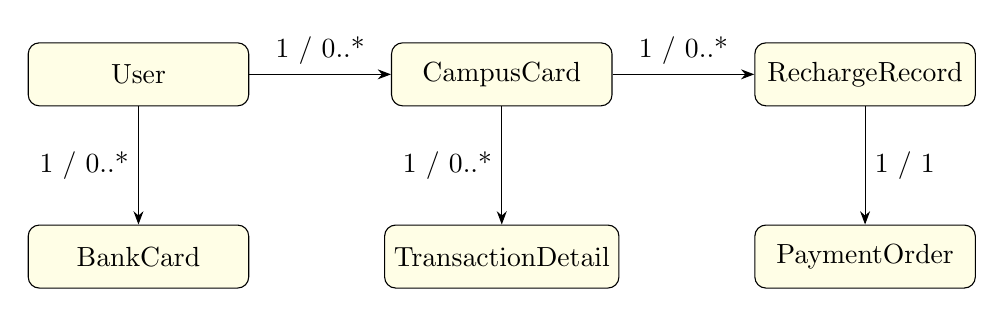
\begin{tikzpicture}[>=Stealth, cls/.style={draw, rounded corners, align=center, minimum width=28mm, minimum height=8mm, fill=yellow!10}, node distance=15mm and 18mm]
\node[cls] (user) {User};
\node[cls, right=of user] (card) {CampusCard};
\node[cls, right=of card] (record) {RechargeRecord};
\node[cls, below=of user] (bank) {BankCard};
\node[cls, below=of card] (detail) {TransactionDetail};
\node[cls, below=of record] (order) {PaymentOrder};
\draw[-{Stealth}] (user) -- node[above]{1 / 0..*} (card);
\draw[-{Stealth}] (user) -- node[left]{1 / 0..*} (bank);
\draw[-{Stealth}] (card) -- node[above]{1 / 0..*} (record);
\draw[-{Stealth}] (card) -- node[left]{1 / 0..*} (detail);
\draw[-{Stealth}] (record) -- node[right]{1 / 1} (order);
\end{tikzpicture}}
\end{center}



充值顺序图：

\begin{center}
\resizebox{1.0\textwidth}{!}{%
\begin{tikzpicture}[>=Stealth, lifeline/.style={dashed, gray}, head/.style={draw, rounded corners, fill=blue!5, align=center, minimum width=24mm, minimum height=7mm}, msg/.style={->, thick}, ret/.style={->, thick, dashed}]
\node[head] (p0) at (0.0,0) {User};
\draw[lifeline] (0.0,-0.35) -- (0.0,-8.60);
\node[head] (p1) at (2.8,0) {RechargePage};
\draw[lifeline] (2.8,-0.35) -- (2.8,-8.60);
\node[head] (p2) at (5.6,0) {Controller};
\draw[lifeline] (5.6,-0.35) -- (5.6,-8.60);
\node[head] (p3) at (8.399999999999999,0) {RechargeService};
\draw[lifeline] (8.399999999999999,-0.35) -- (8.399999999999999,-8.60);
\node[head] (p4) at (11.2,0) {CardRepo};
\draw[lifeline] (11.2,-0.35) -- (11.2,-8.60);
\node[head] (p5) at (14.0,0) {RecordRepo};
\draw[lifeline] (14.0,-0.35) -- (14.0,-8.60);
\node[head] (p6) at (16.799999999999997,0) {PaymentGateway};
\draw[lifeline] (16.799999999999997,-0.35) -- (16.799999999999997,-8.60);
\draw[msg] (0.0,-0.85) -- node[above, font=\scriptsize, align=center] {输入充值金额} (2.8,-0.85);
\draw[msg] (2.8,-1.57) -- node[above, font=\scriptsize, align=center] {POST /recharges} (5.6,-1.57);
\draw[msg] (5.6,-2.29) -- node[above, font=\scriptsize, align=center] {recharge(command)} (8.399999999999999,-2.29);
\draw[msg] (8.399999999999999,-3.01) -- node[above, font=\scriptsize, align=center] {findByCardNo} (11.2,-3.01);
\draw[msg] (8.399999999999999,-3.73) -- node[above, font=\scriptsize, align=center] {pay(amount)} (16.799999999999997,-3.73);
\draw[ret] (16.799999999999997,-4.45) -- node[above, font=\scriptsize, align=center] {success} (8.399999999999999,-4.45);
\draw[msg] (8.399999999999999,-5.17) -- node[above, font=\scriptsize, align=center] {save(card)} (11.2,-5.17);
\draw[msg] (8.399999999999999,-5.89) -- node[above, font=\scriptsize, align=center] {save(record)} (14.0,-5.89);
\draw[ret] (8.399999999999999,-6.61) -- node[above, font=\scriptsize, align=center] {result} (5.6,-6.61);
\draw[ret] (5.6,-7.33) -- node[above, font=\scriptsize, align=center] {JSON} (2.8,-7.33);
\end{tikzpicture}}
\end{center}



\section{SRS 与验收标准}

SRS 条目要能导出测试：

\begin{quote}
\footnotesize
\begin{verbatim}
FR-01 当持卡人提交充值请求时，系统应校验校园卡状态和充值金额。
AC-01 Given 校园卡状态正常且金额为 100 元，
When 持卡人提交充值请求，
Then 系统创建充值订单。
\end{verbatim}
\end{quote}

一个好的需求条目要满足：

\begin{itemize}
\item 有编号。
\item 描述单一行为。
\item 条件清楚。
\item 响应清楚。
\item 可以被测试。
\item 能追踪到设计、代码和测试。
\end{itemize}

\section{自测题与答案}

\section{题 1：需求的分类有哪些？}

答案：

按层次分为业务需求、用户需求、系统级需求。按类型分为功能需求、非功能需求、对外接口需求、约束和数据需求。非功能需求还可细分为性能、安全、可靠性、可维护性、易用性等质量属性。

\section{题 2：需求的层次性是什么？}

答案：

业务需求说明组织为什么建设系统；用户需求说明用户要用系统完成什么任务；系统级需求说明系统在具体输入和条件下必须提供什么行为和响应。三者从目标到任务再到系统规格逐层细化。

\section{题 3：如何改写“所有用户查询都必须在很快的时间内完成”？}

答案：

原表述不可测试，“很快”没有阈值。可改为：

\begin{quote}
\footnotesize
\begin{verbatim}
当用户提交余额查询请求时，
系统应在 2 秒内返回查询结果；
该时间不包含外部支付平台响应时间。
\end{verbatim}
\end{quote}

\section{题 4：什么情况下使用 include，什么情况下使用 extend？}

答案：

多个用例都必须执行同一段公共行为时使用 include；某行为只在特定条件下发生时使用 extend。include 的方向是基本用例指向被包含用例；extend 的方向是扩展用例指向基本用例。

\section{题 5：概念类图和设计类图的区别是什么？}

答案：

概念类图属于需求分析，描述问题域概念、属性、关联和多重性，不写方法和实现细节。设计类图属于详细设计，描述软件类、接口、方法、可见性、继承、依赖和实现结构。

\section{题 6：AI 生成需求模型后要审查什么？}

答案：

审查系统边界、术语一致性、遗漏的异常流程、隐含业务规则、关联方向、多重性、状态迁移条件、需求编号和追踪关系。AI 输出只能作为初稿，最终模型要由工程师根据问题域验证。

\bigskip\hrule\bigskip

\section{快速背诵清单}

\section{需求工程}

\begin{itemize}
\item 活动：获取、分析、规格说明、验证、管理。
\item 层次：业务需求、用户需求、系统级需求。
\item 类型：功能、非功能、接口、约束、数据。
\item 用例：用户目标、参与者、系统边界、include、extend。
\item SRS：系统视角、刺激-响应、可验证、可追踪。
\end{itemize}
\end{document}

